% !TEX root = ../../../main/aws_chabauty.tex
\newpage
\section{Jennifer Balakrishnan: Computational tools for quadratic Chabauty}
\subsection{Lecture 1}
\subsubsection{An Example}

\begin{ques}
Does there exist a pair of rational right triangles and a rational isosceles triangle that have the same area and the same perimeter?
\end{ques}


If the answer to the question was a yes, we could draw triangles of the following form:
	

	\begin{figure}[!ht]
	\centering
	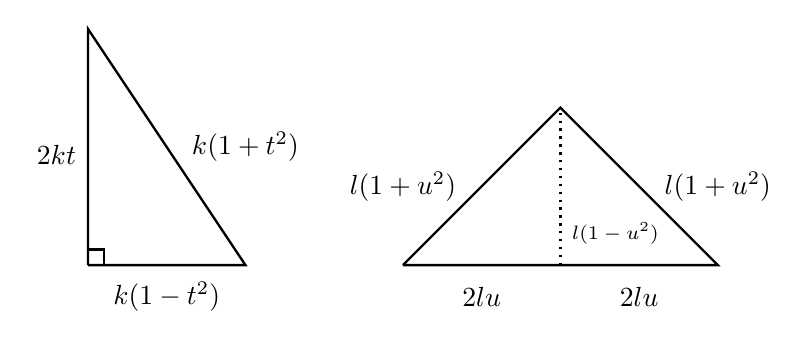
\begin{tikzpicture}
	\draw[line width=0.03cm] (0,0) -- (0,3) -- (2,0) -- (0,0);
	\draw[line width=0.03cm] (0,0.2) -- (0.2,0.2) -- (0.2,0);
	\node at (1,-0.4) {$k(1-t^2)$};
	\node at (-0.4,1.4) {$2kt$};
	\node at (2.0,1.5) {$k(1+t^2)$};
	
	\draw[line width=0.03cm] (4,0) -- (6,2) -- (8,0) -- (4,0);
	\draw[line width=0.03cm,dotted] (6,0) -- (6,2);
	\node at (4,1) {$l(1+u^2)$};
	\node at (8,1) {$l(1+u^2)$};
	\node at (5,-0.4) {$2lu$};
	\node at (7,-0.4) {$2lu$};
	\node at (6.7,0.4) {\scriptsize$l(1-u^2)$};
	\end{tikzpicture}
	\end{figure}


We rescale so that we can assume $l=1$. Now suppose $k,t,u \in \Q$, $0<t,u<1$, and $k>0$. Equating areas and perimeters, we find the simultaneous system of equations 
	\[
	\begin{cases}
	k^2 t (1 - t^2)= 2u (1 - u^2) \\
	k + kt= 1 + 2u + u^2 
	\end{cases}
	\]
After some algebra, we see there exists $x \in \Q$, $1<x<2$, such that $2xk^2+(-3x^2 - 2x^2 + 6x - 4)k + x^5= 0$. The discriminant of this polynomial in $k$ is a rational square. But then for some $y$, we have
	\[
	y^2= (-3x^2 - 2x^2 + 6x - 4)^2 - 4(2x)x^5= x^6 + 12x^5 - 32x^4 + 52x^2 - 48x + 16
	\]
We can then define a curve $X$ by
	\[
	X \colon \quad y^2= x^6 + 12x^5 - 32x^4 + 52x^2 - 48x + 16
	\]
Now $X$ is a genus 2 curve, and we would like to determine $X(\Q)$. The Jacobian, $J$, of $X$ has rank $\rank J(\Q)=1$. Also, the Chabauty-Coleman bound gives $\#X(\Q) \leq 10$. However, we have yet to actually find any rational points! In fact, we can find 
	\[
	\{\infty^\pm, (0,\pm 4), (1,\pm 1), (2, \pm 8), (12/11,\pm 868/11^3) \} \subseteq X(\Q)
	\]
Therefore, we have completely determined $X(\Q)$, and the rational point $(12/11,868/11^3)$ gives us a unique pair of triangles. It was Hirakawa and Matsumura in 2018 that answered this discriminant question, and hence the triangle question, that yes, there are exactly one pair of such triangles.


\begin{thm}[Hirakawa-Matsumura, 2018]
Up to similitude, there exists a unique pair of rational right triangles and a rational isosceles triangle which have the same perimeter and the same area. The unique pair consists of the right triangle with side $(377,135,352)$. and isosceles triangle with sides $(366,366,132)$. 
\end{thm}



% Coleman's Effective Chabauty
\subsubsection{Coleman's Effective Chabauty}

Let $X/\Q$ be a `nice' curve with genus $g \geq 2$. Suppose that $r= \rank J(\Q) < g$. If $p>2g$ is good reduction for $X$, then $\#X(\Q) \leq \#X(\F_p) + 2g - 2$. This bound comes from bounding the number of zeros of a $p$-adic (Coleman) integral. Coleman gave this theory of $p$-adic line integration in the 1980s. In particular, he proved 


\begin{thm}[Coleman]
Let $X/\Qp$ be a nice curve with good reduction at $p$. The $p$-adic integral $\ds\int_P^Q \omega \in \ov{\Q}_p$, defined for $P,Q \in X(\ov{\Q}_p)$ and regular differential $\omega \in H^0(X,\Omega^1)$, satisfies the following:

        \begin{enumerate}[(i)]
        \item the integral is $\ov{\Q}_p$-linear in $\omega$.
        
        \item if $P,Q$ reduce to the same point $\ov{P} \in X(\ov{\F}_p)$, then we call the integral a `tiny' integral. It can be evaluated by writing $\omega= \omega(t) \;dt$, with $t$ is a uniformizer at $\ov{P}$ and $\omega$ a power series, then integrating formally and obtaining a power series $\ell$ such that $d\ell(t)= \omega(t) \;dt$, and finally evaluating $\ell(t(Q))$, which converges. This implies $\ds\int_P^P \omega= 0$.
        
        \item We have
        	\[
        	\int_P^Q \omega + \int_{P'}^{Q'} \omega= \int_P^{Q'} \omega + \int_{P'}^Q \omega
        	\]
	Then it makes sense to define $\ds\int_D \omega$ for 
	\[
	D= \sum_{j=1}^n \big( \, (Q_j) - (P_j)\, \big) \in \div_X^0(\ov{\Q}_p)
	\]
	as 
	\[
	\int_D \omega= \sum_{j=1}^n \int_{Q_j}^{P_j} \omega.
	\]
        
        \item if $D$ is principal, then $\ds\int_D \omega= 0$.
        
        \item The integral is compatible with the action of $\Gal(\ov{\Q}_p/\Qp)$.
        
        \item Fix $P_0 \in X(\ov{\Q}_p)$. If $0 \neq \omega \in H^0(X_{\Qp}, \Omega^1)$, then the set of points $P \in X(\ov{\Q}_p)$ reducing to a fixed point on $X(\F_p)$ such that $\ds\int_{P_0}^{P_1} \omega= 0$ is finite. 
        \end{enumerate}
\end{thm}


The integral above is known as the Coleman integral. Now given the hypotheses of the previous theorem, let $b \in X(\Qp)$, and $J$ be the Jacobian of $X$ with Abel-Jacobi imbedding $i: X \hra J$ given by $P \mapsto [P - b]$. There is a map $J(\Qp) \times H^0(X_{\Qp}, \Omega^1) \to \Qp$ given by $(Q, \omega) \mapsto \langle Q, \omega \rangle$ that is additive in $Q$, $\Qp$-linear in $\omega$, and given by 
	\[
	\langle [D], \omega \rangle= \int_D \omega \text{ for } D \in \div_X^0.
	\]


But then for $P \in X(\Qp)$, we have the Abel-Jacobi morphism $\abj_b$ that takes $P$ to the linear functional
	\[
	\langle i(P), \omega \rangle= \int_b^P \omega =: \abj_b(P).
	\]
The Chabauty-Coleman method uses a certain subspace of the space of regular 1-forms. We will assume that $b \in X(\Q)$, and use this to embed $X \hra J$.


\begin{dfn}[Annihilating Differentials]
Let $A= \{ \omega \in H^0(X, \Omega^1) \colon \text{ for all } P \in J(\Q), \langle P, \omega \rangle= 0 \}$ is the subspace of annihilating differentials.  
\end{dfn}


The embedding $i: X \hra J$ induces an isomorphism of vector spaces $H^0(J_{\Qp}, \Omega^1) \simeq H^0(X_{\Qp}, \Omega^1)$. Similarly, we have a pairing $J(\Qp) \times H^0(J_{\Qp}, \Omega^1) \ma{} \Qp$ given by $\ds (Q, \omega_J) \mapsto \int_0^Q \omega_J$. This induces a homomorphism $\log: J(\Qp) \to H^0(J_{\Qp}, \Omega^1)^*$. Thus, we have the following diagram
	\[
	\begin{tikzcd}
	X(\Q) \arrow{d} \arrow{r} & X(\Qp) \arrow{d} \arrow{dr}{\abj_b} \\
	J(\Q) \arrow{r} & J(\Qp) \arrow{r}{\log} &  H^0(J_{\Qp},\Omega^1)^* \simeq H^0(X_{\Qp}, \Omega^1)^*
	\end{tikzcd}
	\]
By ``computing rational points via the Chabauty-Coleman method'', we mean that we compute the finite set of $p$-adic points
	\[
	X(\Qp)_1:= \{ z \in X(\Qp) \colon \int_b^z \omega= 0 \text{ for all } \omega \in A \}.
	\]
By construction, $X(\Q) \subset X(\Qp)$. Of course, it might be that $X(\Qp)_1$ is strictly larger than a known set of rational points in $X(\Q)$, so that extra work needs to be done in order to provably compute $X(\Q)$ entirely. One approach to this problem is the Mordell-Weil sieve. But how do we compute the annihilating differential? 


\begin{ex}
Let $X: y^2= x^5 - 2x^3 + x + \frac{1}{4}$, which has LMFBD label \href{https://www.lmfdb.org/Genus2Curve/Q/971/a/971/1}{971.a.971.1}. Here are some facts about $X$:

\begin{enumerate}[(i)]
\item $X(\Q)_{\text{known}}= \{ \infty, (0,\pm1/2), (-1,\pm1/2), (1,\pm 1/2) \}$.

\item $J$ is simple, $J(\Q) \simeq \Z$, and the point $[(-1,-1/2)-(0,1/2)] \in J(\Q)$ has infinite order (this can be seen by computing the Coleman integrals on regular 1-forms). 

\item The conductor $N$ is 971, which is prime. Therefore, $X$ has good reduction at $p=3$, and we can compute $\#X(\F_3)=7$. Using Stoll's refinement of the Chabauty-Coleman bound for $p= 3$, we find
	\[
	\#X(\Q) \leq \#X(\F_3) + 2 r + \floor*{\dfrac{2 \cdot 1}{3  - 2}} = 11
	\]
\end{enumerate}
This bound is then now sharp enough to prove that we have all the $\Q$-points. [In fact, we do not even know that we have all the $\Q$-points, though we suspect this is the case, and it is. We would like to prove this.]

We will use $p= 3$ to construct a 3-adic annihilating differential $\eta$. A basis of $H^0(X_{\Qp},\Omega^1)$ is 
	\[
	\left\{ \omega_i = \dfrac{x^i \;dx}{2y} \right\}_{i=0,1}.
	\]
So $\eta$ is a $\Q_3$-linear combination of $\omega_0, \omega_1$. We will compute the values of 
	\begin{flalign}
	&& \alpha&:= \int_{(0,1/2)}^{(-1,-1/2)} \omega_0 && \notag \\
	\text{and} && \phantom{x} & \phantom{x} && \notag \\
	&& \beta&:= \int_{(0,1/2)}^{(-1,-1/2)} \omega_1 && \notag
	\end{flalign}
to compute $\eta$. SageMath can compute $\alpha, \beta$
	\[
	\begin{aligned}
	\alpha&= 3 + 3^2 + 3^4 + 3^5 + 2 \cdot 3^6 + 2 \cdot 3^7 + 2 \cdot 3^8 + 3^{10} + O(3^{11}) \\
	\beta&= 2 + 2\cdot 3 + 2 \cdot 3^2 + 2 \cdot 3^3 + 3^4 + 3^6 + 2 \cdot 3^8 + 2 \cdot 3^9 +  O(3^{10}). 
	\end{aligned}
	\]
Taking a slightly different basis (see the notes), we can take $\eta= \beta \omega_0 - \alpha \omega_1$ as our annihilating differential and run Chabauty-Coleman.\footnote{Note, use Sage for hyperelliptic curves and Magma for plane curves.}
\end{ex}



% Explicit Coleman Integration
\subsubsection{Explicit Coleman Integration}

But where do all these numbers come from? They come from using the action of Frobenius on $p$-adic cohomology. Let $X^\an$ denote the rigid analytic space over $\Qp$ associated to $X/\Qp$. 


\begin{dfn}[Wide Open Subspace]
A wide open subspace of $X^\an$ is the complement in $X^\an$ of the union of a finite collection of disjoint closed disks of radius $\lambda_i < 1$.
\end{dfn}


Before continuing, we will give a few more properties of the Coleman integral that we will need. 


\begin{thm}[Coleman]
Let $\eta, \xi$ be 1-forms on a wide open subspace $V$ of $X^\an$, and let $P,Q, R \in V(\ov{\Qp})$. Let $a,b \in \ov{\Qp}$. Then we have 

\begin{enumerate}[(i)]
\item Linearity in the integrand:
	\[
	\int_P^Q (a\eta + b \xi)= a \int_P^Q \eta + b \int_P^Q \xi
	\]

\item Additivity in the endpoints:
	\[
	\int_P^R \eta + \int_R^Q \eta= \int_P^Q \eta
	\]

\item Change of variables under rigid analytic maps (Frobenius): if $V' \subset X'$ is a wide open subspace of the rigid analytic space $X', \omega'$, a 1-form on $V'$ and $\phi: V \to V'$ a rigid analytic map, then
	\[
	\int_P^Q \phi^* \omega'= \int_{\phi(P)}^{\phi(Q)} \omega'. 
	\]

\item Fundamental Theorem of Calculus:
	\[
	\int_P^Q \;df= f(P) - f(Q)
	\]
for a rigid analytic function on $V$.

\item Galois compatibility: if $P,Q \in V(\Qp)$ and $\omega$ is defined over $\Qp$, then $\ds \int_P^Q \omega \in \Qp$. 
\end{enumerate}
\end{thm}


We first integrate $\int_P^Q \omega$ for $\omega$ a 1-form of the second kind, where $P, Q \in V(\Qp)$. We will discuss this in the case where $X$ is a hyperelliptic curve by examining the method of explicit Coleman integration due to Balakrishnan-Bradshaw-Kedlaya. The method is the following: \par\vspace{\baselineskip}


\noindent\makebox[\textwidth][c]{%
\begin{minipage}{0.8\textwidth}
\begin{enumerate}[1.]
\item Take a lift, $\phi$, of $p$-power Frobenius from the special fiber.
\item Compute a basis, $\{ \omega_i \}$, of 1-forms of the second kind.
\item Compute $\phi^* \omega_i$ via Kedlaya's zeta function algorithm, and use properties of Coleman integrals to relate $\ds \int_P^Q \phi^*\omega_i$ to $\ds \int_P^Q \omega_i$ and other terms.
\item Solve for $\int_P^Q \omega_i$ using linear algebra.
\end{enumerate}
\end{minipage}%
} \par\vspace{\baselineskip}
 

We sketch Kedlaya's algorithm. Let $X$ be the curve $y^2= p(x)$. We work in an affine $Y \subset X$ given by defining Weierstrass points. Take $\phi$ to be $x \mapsto x^p$ and $\ds y \mapsto y^p \sum_{j=0}^\infty \binom{1/2}{1} \left( \dfrac{p(x^p - p(x)^p}{y^{2p}} \right)^j$. Then we compute the action of $\phi$ on
	\[
	\begin{aligned}
	\phi^*\left( \dfrac{x^i \;dx}{y} \right)&= \dfrac{x^{pi} \;d(x^p)}{\phi(y)} \\
	&= \dfrac{x^{pi} p x^{p-1} \;dx}{\phi(y)} \\
	&= p x^{pi + p - 1} y^{-p} \sum_{j=0}^\infty \binom{1/2}{1} \left( \dfrac{p(x^p - p(x)^p}{y^{2p}} \right)^j
	\end{aligned}
	\]
and reduce pole order of each resulting differential using relations in $H^1$. Denote the basis by $\{\omega_i\}_{i=0,\ldots,2g-1}$. Then Kedlaya's algorithm gives
	\[
	\phi^* \omega_i= dh_i + \sum_{j=0}^{2g-1} \mu_{ji} \omega_j
	\]
If we can compute $h_i$ and $M$, then
	\begin{equation} \label{eq:balk_star}
	\begin{pmatrix}
	\vdots \\
	\ds \int_P^Q \omega_i \\
	\vdots
	\end{pmatrix}=
	(M^t - I)^{-1} 
	\begin{pmatrix}
	\vdots \\
	\ds h_i(P) - h_i(Q) - \int_P^{\phi(P)} \omega_i - \int_{\phi(Q)}^Q \omega_i \\
	\vdots
	\end{pmatrix} 
	\tag{*}
	\end{equation}


Finishing the 3-adic integrals on $y^2= x^5 - 2x^3 + x + 1/4$, we constructed $\eta= \beta \omega_0 - \alpha \omega_1$, where $\alpha,\beta$ are computed using \eqref{eq:balk_star}. We want to compute $X(\Q_3)_1$. Note that $X(\F_3)= \{ \infty, (0,\pm1), (1,\pm 1),(2\pm1) \}$. We need to compute power series expansions of
	\[
	\left\{ \int_{(0,1/2)}^{P_t} \eta \right\}
	\]
where $P_t$ ranges over all residue disks, and then solve for $z \in X(\Q_3)$ such that $\ds \int_{(0,1/2)}^z \eta= 0$. To compute these integrals, we can take $P_0$ to be a lift of some $\F_3$-point in the same residue disk as $P_t$. Then
	\[
	\int_{(0,1/2)}^{P_t} \eta= \underbrace{\int_{(0,1/2)}^{P_0} \eta}_{\text{Gives 3-adic}} + \underbrace{\int_{P_0}^{P_t} \eta}_{\text{Coleman 3-adic series}}
	\]
Note the first integral on the right side is some 3-adic constant, and the second is a tiny integral which was computed using a local coordinate at $P_0$. As a lucky fact, for each residue disk, there exists a rational point $P_0 \in X(\Q)$ such that the 3-adic number is 0. This forces the constant of integration to be 0 in each residue disk by the construction of the annihilating differential. Then any further computation is solely local. Computing the tiny integral in each residue disk, we find each just has a simple zero at a known rational point, and no others. But then we have
	\[
	X(\Q_3)_1= X(\Q)_{\text{known}}= \{ \infty, (0,\pm 1/2), (-1,\pm1/2), (1,\pm 1/20 \}
	\]
which proves that $\#X(\Q)= 7$. 

 